\chapter{Methods}

In this chapter, we discuss our solution to the problem of predicting solar power production. We cover the data we had access to and ultimately selected to train the neural network with, and how we processed and structured the data. We explain the Temporal Fusion Transformer architecture and how we set it up and use it to achieve our goals.

\section{Data}
This work relies on two types of data, \emph{the ground truth}, the measured irradiance at the power station and \emph{the input}, the irradiance values from high-resolution weather forecasts for the area. The data spans the 425 days from August 1st 2020 to September 30th 2021 for the Ituverava solar power station run by Enel S.p.A. in Minas Gerais, Brazil.

\subsection{Irradiance measurements}
Under certain circumstances irradiance values simulated after the fact can be accurate, however this does not apply in all conditions, and real measured values are much more reliable \cite{gueymard_global_2008}. The irradiance was measured with seven Kipp \& Zonen CM21 pyranometers placed around the power station. The pyranometers have a reported maximum measurement error of 3\%. For input into the network, the highest and lowest measured values are dropped and the average value of the other five measurements is used. This data is provided with five-minute intervals, but the neural network operates hourly. To downsample the measurement data to an hourly format, we averaged the values for the twenty minutes before and after the beginning of each hour. Finally, the irradiance values were normalized linearly to the range $0.0-1.0$ before being input into the neural network.


\subsection{Forecast Data\label{cha:forecast_data}}
The weather forecast data is provided by Belgingur ehf., Reykjavík, Iceland. We use irradiance values from historical 24-hour weather forecasts generated by their WRF model, discussed in Section~\ref{cha:WRF}. The forecasts have a temporal resolution of one hour and a spatial resolution of 2.5km. One of our models uses forecast data from a 3x3 grid centred on the solar power station, and the other model the data from only the centre of the grid. We use two irradiance values from the forecast, the downward irradiance and the downward diffuse irradiance. These irradiance values were normalized linearly to the range $0.0-1.0$ before being input into the neural network.


\subsection{Error metric}
In other work done in this area, multiple error metrics are used. One error metric is used more commonly than others, Mean Absolute Percentage Error (MAPE) \cite{lin_temporal_2020, lee_forecasting_2018, jaidee_very_2019, su_machine_2019}, which is the reason that metric was chosen.
When working with near-zero values MAPE becomes unhelpful as it is calculated by dividing by that near-zero value, so all cases where the irradiance is less than 15\% of the maximum value in the data set are dropped. Hence we do not evaluate early morning or late evening performance.
While a valuable metric, MAPE does not  fully represent the function of the model. Other factors like confidence, discussed in Section~\ref{sec:loss_function} and deviance from total irradiance for the day also represent key factors in the usefulness of the model.




\section{Tools}
The neural network was implemented in PyTorch 1.11 and PyTorch Forecasting 0.9.0. We used an NVIDIA GeForce RTX 3080Ti graphics card using CUDA for training. The computer had an AMD Ryzen 9 5950X CPU, 32GB of RAM and was running Windows 11.
This allowed for quick training of models, as with the relatively small amount of data, training a model took 5-10 minutes.


\section{Model}
    \subsection{Temporal Fusion Transformer}
    
    \noindent We utilize a Temporal Fusion Transformer (TFT) model for the irradiance prediction.
    TFTs are  general networks which use attention at their core to generate multi-horizon forecasts with the ability to consider
    known information about the future, other related time series, and static metadata for the forecast \cite{lim_temporal_2020}. Figure~\ref{fig:tft_overviwew} shows an overview of how TFTs operate.
    
    \afterpage{%
    \begin{figure}
        \centering
         \makebox[\textwidth][c]{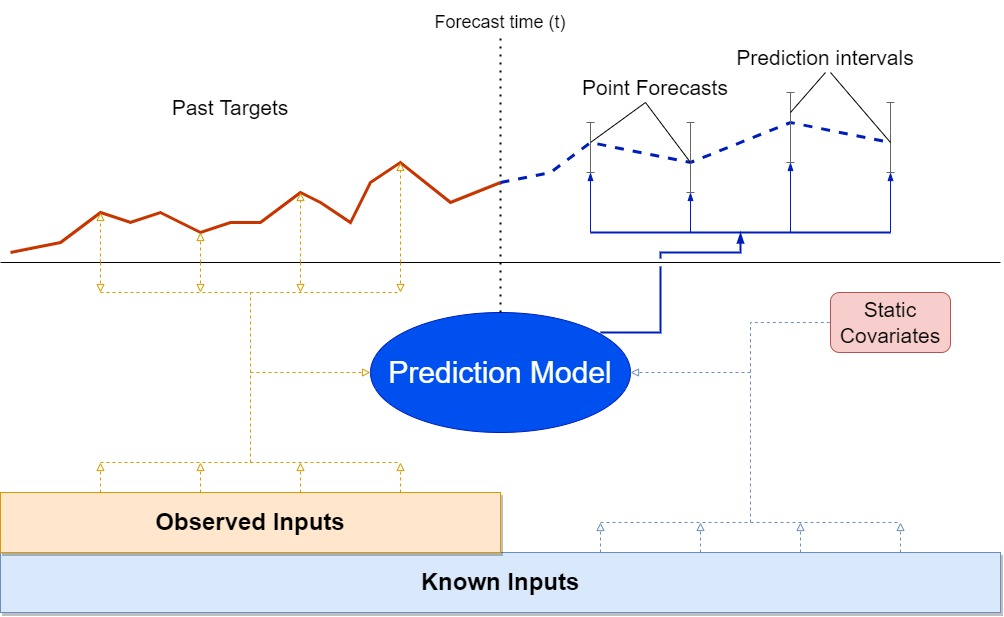
\includegraphics[scale=0.5]{imgs/TFT_overview.jpg}}
        \caption{An overview of the Temporal Fusion Transformer.
        \label{fig:tft_overviwew}}
    \end{figure}
    \clearpage
    }
    
    \noindent TFTs are composed of various components, each primarily addressing a single input type (i.e. static, known or observed inputs), aimed at maximizing the model versatility across various problems.
    

    
    \noindent\textbf{Gating mechanisms} identify and skip unused input data, granting models greater ability to work with less curated input data, or datasets where it is unknown which parts are of significance.\\
    The Gated Residual Network (GRN) structure, shown in Figure~\ref{fig:ttgt_detail}, is a base building block of TFTs \cite{lim_temporal_2020}. It provides the model the flexibility to choose the complexity of its input, more complex where needed, and less complex where not.\\
    \clearpage
    \noindent\textbf{Variable selection networks} emphasize the most relevant inputs for every time step \cite{lim_temporal_2020}. Some variables may be more important than others, \enquote{TFT is designed to provide instance-wise variable selection through the use of variable selection networks applied to both static covariates and time-dependent covariates.} \cite{lim_temporal_2020} The variable selection mechanism also allows the model to remove noisy inputs that might have a negative effect on performance. \\
    \textbf{Static covariate encoders} encode static features into context vectors, integrating them into the network \cite{lim_temporal_2020}.  \\
    \textbf{Temporal processing} using a more traditional RNN sequence-to-sequence layer (see Section~\ref{cha:RNN}) for short term, local processing and the more novel multi-headed attention layer (see Section~\ref{cha:transformer}) for long term pattern capture \cite{lim_temporal_2020}.\\
    \textbf{Prediction intervals} in the form of quantile forecasts, discussed in Section~\ref{sec:loss_function}, display a confidence interval for the predictions \cite{lim_temporal_2020}. \\
    Figure~\ref{fig:ttgt_detail} shows a detailed view of the TFT structure as discussed. 
    
    \afterpage{%
    \begin{figure}
        \centering
         \makebox[\textwidth][c]{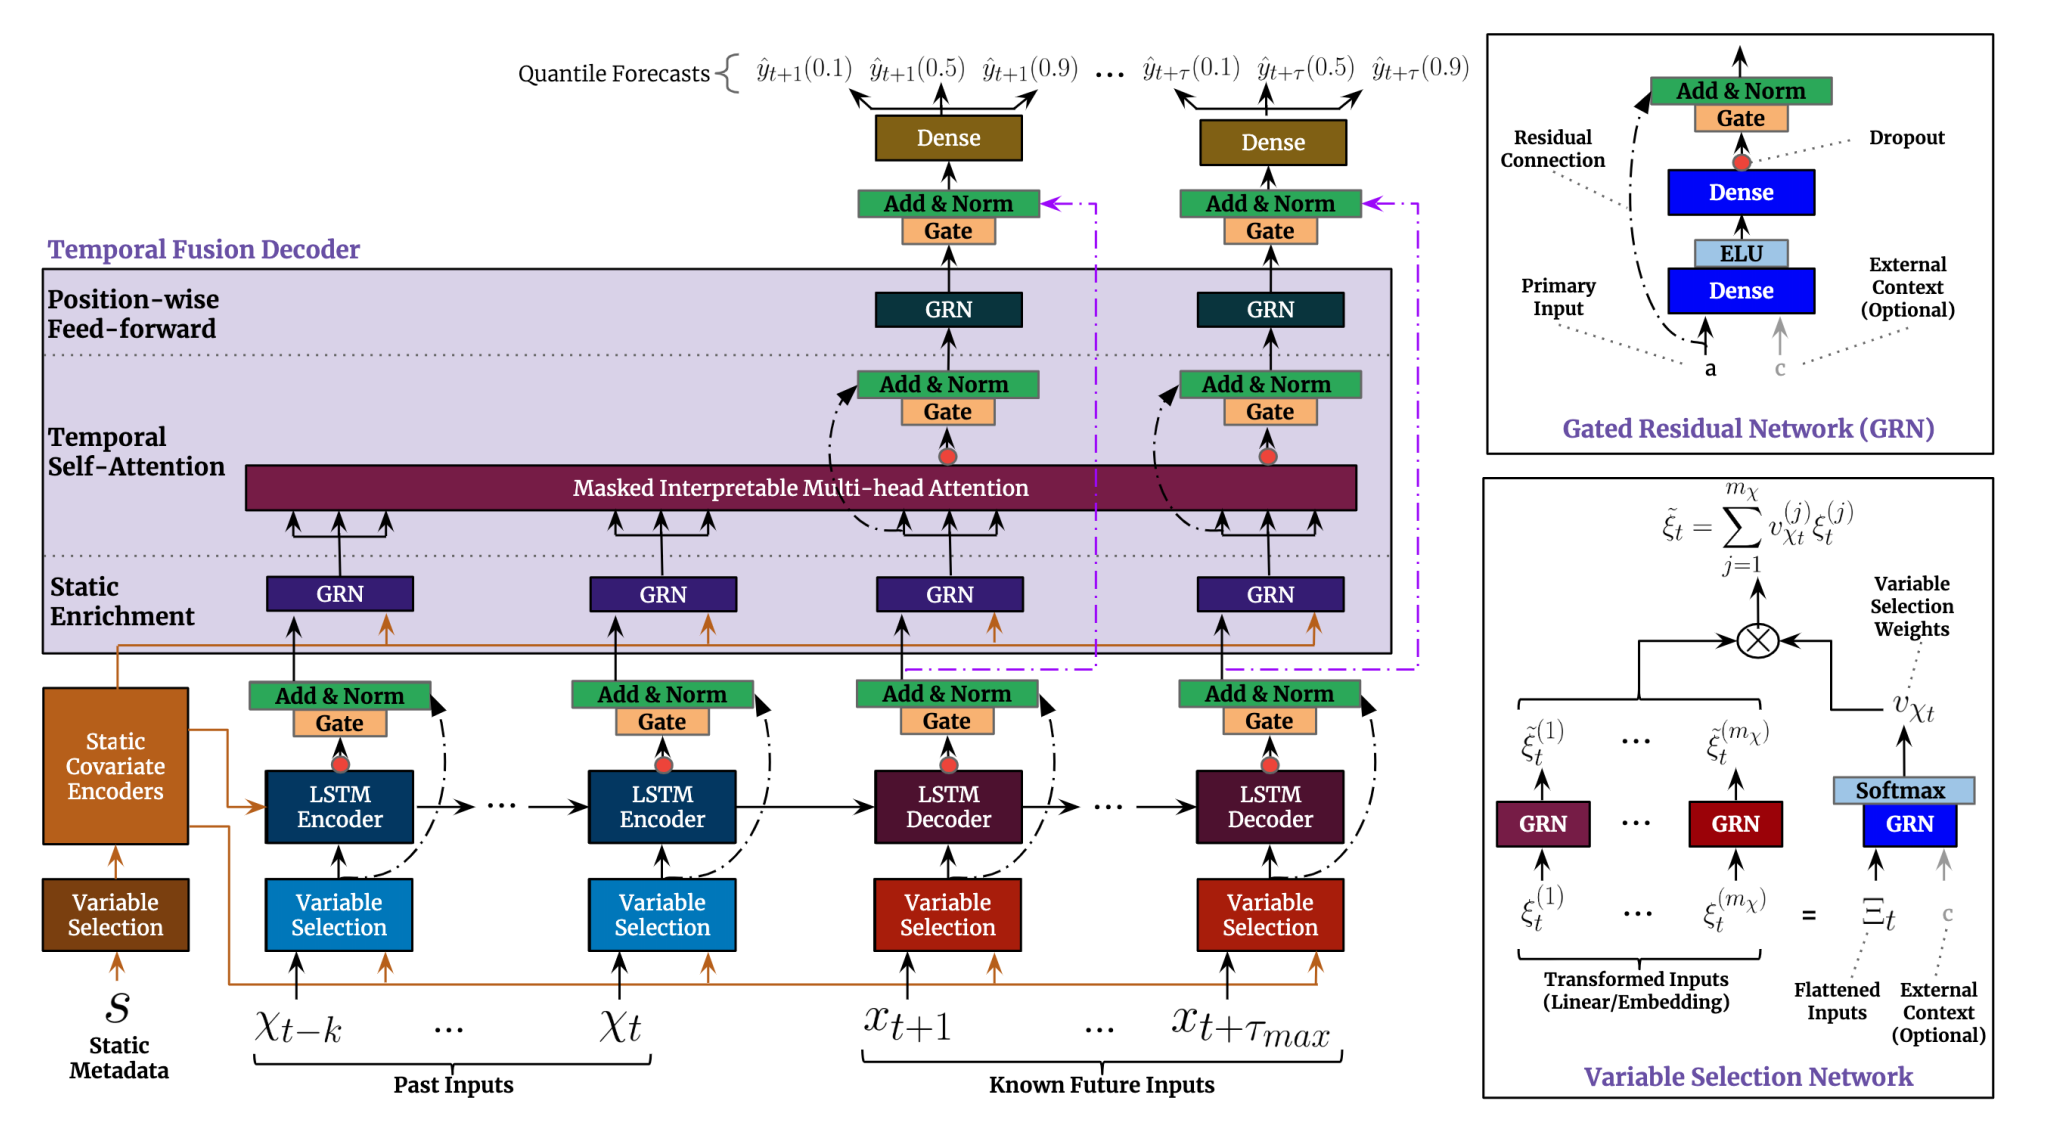
\includegraphics[scale=0.36]{imgs/TFT.png}}
        \caption{A detailed view of the architecture of the Temporal Fusion transformer.\cite{lim_temporal_2020}
        \label{fig:ttgt_detail}}
    \end{figure}
    \clearpage
    }

    \subsection{Setup}
    We trained two models. One which utilizes weather forecast data from an area surrounding the power station, and one which does not, as discussed in Section~\ref{cha:forecast_data}. The limited model is intended to show that the full model is able to glean additional information from the surrounding area data.
    
    
    \afterpage{%
    \begin{figure}
        \centering
        \makebox[\textwidth][c]{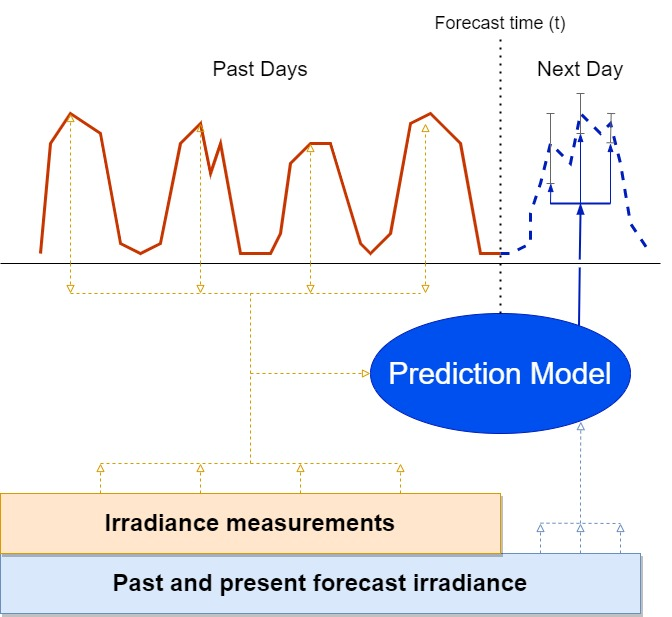
\includegraphics[scale=0.6]{imgs/solar_TFT_overview.jpg}}
        \caption{An overview of the setup of the neural network.
        \label{fig:solar_tft_overviwew}}
    \end{figure}
    \clearpage
    }


    \subsubsection{Inputs}
        The dataset was split into a training set, composing 70\% of the data, a validation set, composing 10\% of the data and finally, 20\% of the data was reserved for testing.
        Figure~\ref{fig:solar_tft_overviwew} shows how the observed inputs, the irradiance measurements, along with corresponding data from historical irradiance forecasts are used as training inputs.
        
    \pagebreak
    \subsubsection{Tuning}
        Significant tuning was done to optimize the performance of both models. Since the goal of tuning was not only to minimize Mean Absolute Percentage Error but balance that with the ability to recognize uncertainty, the process was very manual. Tables~\ref{tab:full_params} and \ref{tab:lim_params} show the selected hyperparameters for the full and limited models respectively.\\
        
        To avoid overfitting and to speed up the training of models, we used early stopping to stop training when the loss function optimization plateaued. 
        
        \vspace{1.5cm}
    
        \begin{table}[ht!]
        \begin{center}
        \caption{The full model hyperparameters.
        \label{tab:full_params}}
        \vspace{0.5cm}
        \begin{tabular}{|l|r|}
        \hline
        \textbf{Hyperparameter} & \textbf{Value} \\ \hline
        Learning rate            & 0.01         \\ \hline
        Batch size              & 24            \\ \hline
        Dropout                 & 0.1            \\ \hline
        Gradient clip           & 0.1           \\ \hline
        Hidden layer size            & 64         \\ \hline
        Hidden continuous size & 8         \\ \hline
        Attention head size   & 1         \\ \hline
        \end{tabular}
        
        \end{center}
        \end{table}
        
        \begin{table}[ht!]
        \begin{center}
        \caption{The limited model hyperparameters.
        \label{tab:lim_params}}
        \vspace{0.5cm}
        \begin{tabular}{|l|r|}
        \hline
        \textbf{Hyperparameter} & \textbf{Value} \\ \hline
        Learning rate            & 0.005         \\ \hline
        Batch size              & 24            \\ \hline
        Dropout                 & 0.1            \\ \hline
        Gradient clip           & 0.1           \\ \hline
        Hidden layer size            & 40         \\ \hline
        Hidden continuous size & 6         \\ \hline
        Attention head size    & 1         \\ \hline
        \end{tabular}
        
        \end{center}
        \end{table}
    
    \pagebreak
    \subsubsection{Loss function}\label{sec:loss_function}
    The loss function used for Temporal Fusion Transformers is quantile loss, as it's an integral part of generating the confidence intervals of the model \cite{lim_temporal_2020}.
    A model's prediction is a random value within a probability distribution \cite{wen_multi-horizon_2018}. If we make multiple predictions we can estimate this probability distribution by seeing within what range a selected proportion of the predictions fall \cite{koenker_quantile_2001}. PyTorch Forecasting's quantile loss function takes the Mean Absolute Error (MAE) of three quantiles, 90\%, 50\% and 10\%. This gives a good picture of the model's confidence in a prediction. A smaller quantile range indicates more confidence.
    
    
    